\documentclass[../uilmath.tex]{subfiles}
\graphicspath{{\subfix{../figures/}}}
\begin{document}
\chapter{Algebra}
\section*{Problems}
\begin{enumerate}[label=\bfseries\arabic*.]
    \item %% Problem 1 
    Evaluate: $1\times (2+3)^{-1}-4\div \frac{5}{6}+7\times(8)^0$
    
    \item %% Problem 2
    If $x$ is $40\%$ less than $y$ and $y$ is $30\%$ more than $z$, then $x$ is \blank than $z$.

    \item %% Problem 3
    Mora Doe goes to the 25\% off book sale. She buys 
    4 romantic novels which cost \$11.95 each before the sale 
    and includes tax. She gave the clerk 2 twenty-dollar bills. How much change should Mora receive?

    \item %% Problem 4
    If $9x^2-12x+4=(ax-b)^2$ then $a+b=\blank$.
    
    \item %% Problem 5
    Harry Hare drove 210 km to Myrtle Turtle's house. Part of the 4 hour trip was in town at 30 km/h 
    and the rest was on a major highway at 60 km/h. How many km did Harry drive on the major highway?

    \item %% Problem 6
    Simplify: $\log_b (3xy)-\log_b(\frac{3x}{2y})+\log_b (3y^2)$

    \item %% Problem 7
    Line $m$ goes through points $(1,-1)$ and $(-3,1)$. Line $n$ goes through points $(1,1)$ and $(x,y)$. Which of the following points lies on line $n$ if $m\perp n$?

    \item %% Problem 8
    Which of the equations will produce the shaded portion of the graph shown?
    \begin{center}
        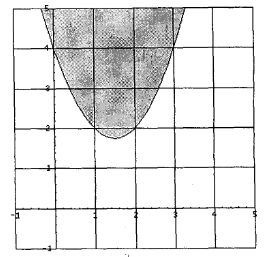
\includegraphics[width=0.3\textwidth]{2006SAC13.PNG}
    \end{center}

    \item %% Problem 9
    The first five terms of an infinite arithmetic sequence is $6\frac{1}{4},A,B,C,12\frac{1}{2},\dots$. Find $A+B+C$.

    \item %% Problem 10
    The numbers of integers that satisfy the inequality new $\frac{3}{7}<\frac{n}{14}<\frac{2}{3}$ is: 

    \item %% Problem 11 
    Define $n\star$ to be $n^n$. Compute $(2\star)\star$.

    \item %% Problem 12
    Evaluate: $\frac{3}{8}\div .75\times \frac{1}{2}-.25+\frac{1}{16}$

    \item %% Problem 13 
    A legend on a map shows 2.5 cm representing 200 miles. The distance on the map from El Paso to Texarkana is 9.8 cm. According to the map, how far is it from El Paso to Texarkana?

    \item %% Problem 14
    Phil Errup's car has a gas tank with a capacity of 18 gallons. The gauge shows that it is $\frac{1}{4}$ full. How many gallons will need to be added to the tank so that it is 75\% full?

    \item %% Problem 15
    Find the equation of the line shown.
    \begin{center}
        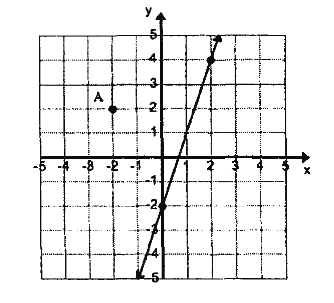
\includegraphics[width=0.3\textwidth]{2008SAC4.PNG}
    \end{center}

    \item %% Problem 16
    Let $p$ and $q$ be the roots of $8x^2+2x-15=0$. Find $p^3+3p^2q+3pq^2+q^3$.

    \item %% Problem 17
    One of the factors of $x^3-3x^2-3x+18$ is: 

    $\textbf{(A)} x+2 \qquad \textbf{(B)} x+3 \qquad \textbf{(C)} x+6 \qquad \textbf{(D)} x-2 \qquad \textbf{(E)} x-9$

    \item %% Problem 18
    The roots of the equation $x^3-5x^2+cx+24=0$ are $3,4$, and $R$. Find $c$.

    \item %% Problem 19
    Let $f(x)=2x+5$ and $g(x)=3x-4$ and $h(x)=6x$. Find $f(g(h(-1)))$.

    \item %% Problem 20
    The coefficient of the 2nd term of the expansion of $(3x-4)^5$ is: 

    \item %% Problem 21
    Solve for $k$ if $3k-4=28-5k$

    \item %% Problem 22
    Joe's dad sent him to the Burger Barn with three twenty-dollar bills and one five-dollar bill. He ordered 6 
    cheeseburgers for \$4.85 each, one basket of fries for \$5.75, 6 large cokes for \$2.19 each and 6 lemon pies for \$1.25 each.
    The tax rate is 8.25\%. How much change did he receive?

    \item %% Problem 23
    Consider a line that is perpendicular to $\overline{BC}$ and also contains point $A$. If the $x$-intercept of ths line is $(a,0)$, then $a=\blank$.
    \begin{center}
        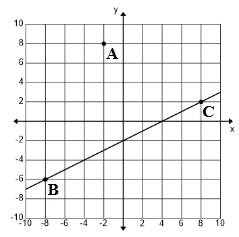
\includegraphics[width=0.3\textwidth]{2021SAC3.PNG}
    \end{center}

    \item %% Problem 24
    The Reagan High math/science team brought in the Quebe Sisters for a UIL fundraiser. Their fee to appear was \$5,000.
    Their version of ``San Antonio Rose'' is outstanding. A student ticket cost \$8.00 and an adult ticket cost \$15.00. A total of 
    2100 tickets were sold and \$20.375 was raised after paying the fee. How many adult tickets were sold?

    \item %% Problem 25
    Consider four consecutive even integers, all positive, such that five times the sum of the first two exceeds three times the sum of the first and fourth by 80. The third integer is \blank.

    \item %% Problem 26
    Simplify: $\frac{\frac{c}{w}+\frac{d}{w^2}}{\frac{m}{w^2}+\frac{k}{hw}}$

    \item %% Problem 27
    If $f(x)=x^2+4$ and $h(x)=3x-1$, then $f(h(5))=\blank$.

    \item %% Problem 28
    Find the number that is $\frac{5}{6}$ of the way from $-4\frac{1}{2}$ to $9\frac{3}{8}$.

    \item %% Problem 29
    Cindy rode her bike for 60 miles at 24 mph and then rode 36 miles at 30 mph. How fast does she need to ride 
    the final 44 miles to have an overall speed of 28 mph? (nearest tenth)

    \item %% Problem 30
    Consider the points $A(-6,10)$ and $B(4,-6)$. Find the equation of a line that exists such that every point on the line 
    is the same distance from $A$ as it is from $B$.

    \item %% Problem 31
    \begin{center}
        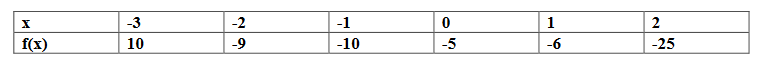
\includegraphics[width=0.3\textwidth]{2021SAC26.PNG}
    \end{center}

    Find the value of $f(-4)$.

    \item %% Problem 32
    If $s(x)$ is the slant asymptote of $h(x)=\frac{x^3+6}{2x^2+x-1}$, then $h(20)-s(20)=\blank$. (nearest thousandth)

    \item %% Problem 33
    If $(x^3-9x^2+kx-12)\div(x-1)$ has a remainder of zero, then $k=\blank$.

    \item %% Problem 34
    Consider the sequence $3,5,8,11,15,20,27,37,m,n,111,\dots$ $m+n=\blank$

    \item %% Problem 35
    Find the distance between the points $(3,5,7)$ and $(-4,1,-3)$. (nearest tenth)

    \item %% Problem 36
    Jeremy has 49 coins with a total value of \$7.05. He only has nickels, dimes, and quarters. He has three more quarters than nickels. How many dimes does he have?

    \item %% Problem 37
    Find the distance between point $A$ and the line shown on the right. (nearest tenth)
    \begin{center}
        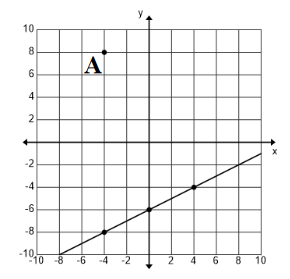
\includegraphics[width=0.3\textwidth]{2021SAC60.PNG}
    \end{center}

    \item %% Problem 38
    At Babe's in Sanger, we ordered four smoked chicken dinners for \$17.95 each, four iced teas for \$2.29 each and two 
    slices of apple pie for \$4.25 each. The tax rate was 8.125\% and I paid with one \$100 bill and one \$20 bill. I told the waitress to 
    keep the change as a tip. How much was her tip?

    \item %% Problem 39
    Consider the line with points $(-3,-5)$ and $(5,7)$. The line contains the point $(0,b)$. $b=\blank$.

    \item %% Problem 40
    Joe sets the motor of his small boat to travel at its maximum speed. At this setting, he travels 36 miles upstream, against the current, in 9 hours 
    and then turns around and travels 36 miles downstream, with the current, in 6 hours. What is the maximum speed of Joe's boat in still water?

    \item %% Problem 41
    Last summer, we drove from Lubbock, TX to McMinnville, OR to see relatives. On day 1, we drove 600 miles at an average speed of 
    62 mph. On day 2, we drove 620 miles at an average speed of 68 mph. On day 3, we drove 534 miles at an average speed of 60 mph. What was our overall average speed for the trip? (nearest tenth)

    \item %% Problem 42
    Jim can clean my pool in 75 min. Tom can clean my pool in 90 min. Julie can clean my pool in 60 min. If all three of them work together, how long would it take them to clean my pool? (nearest tenth)

    \item %% Problem 43
    Consider the line $y=f(x)$ which contains point $P$ and is parallel to the line shown below. Find the value of $f(9)$.

    \begin{center}
        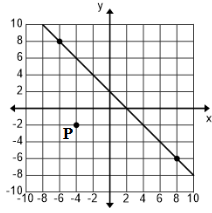
\includegraphics[width=0.3\textwidth]{2022SAC6.PNG}
    \end{center}

    \item %% Problem 44
    The UIL students at Latexo High School sold 246 tickets to the end of the year banquet. If adult tickets cost 
    \$18, student tickets cost \$12, and \$3816 was raised, how many student tickets were sold?

    \item %% Problem 45
    Mary has 57 coins that are either nickels, dimes or quarters. The value of the coins is \$8.60. She has ten more quarters than nickels. How many dimes does she have?

    \item %% Problem 46
    Find the number that is $\frac{3}{4}$ of the way from $-1\frac{1}{2}$ to $6\frac{5}{8}$.

    \item %% Problem 47
    If $f(x)=\frac{2x+5}{3-7x}$, then $f^{-1}(2)=\blank$.

    \item %% Problem 48
    Sixty workers could do 9 jobs in 6 days. How many days would it take 10 workers to do 12 jobs? (nearest tenth)

    \item %% Problem 49
    Consider the line $y=f(x)$ such that all points on the line are equidistant from the points $(-6,8)$ and $(4,-6)$. The $y$-intercept of the line $y=f(x)$ is $(0,b)$. $b=\blank$.

    \item %% Problem 50
    Find the domain of the function $f(x)=\frac{\sqrt{3+x}}{x^2-9x+20}$.

    \item %% Problem 51
    Solve the system 
    \begin{align*}
        \frac{2}{5}a+\frac{3}{10}c=2\frac{1}{5}\\
        -.5a+1.5b=2.5
        .75a-2.5c=-2
    \end{align*}
    $b=\blank$.

    \item %% Problem 52
    The points of intersection of the curves shown on the right are $P$ and $Q$. $PQ=\blank$. (nearest tenth)
    \begin{center}
        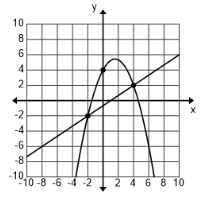
\includegraphics[width=0.3\textwidth]{2022SAC40.PNG}
    \end{center}

    \item %% Problem 53
    
\end{enumerate}

\section*{Solutions}
\begin{enumerate}[label=\bfseries\arabic*.]
    \item %% Problem 1
    $2 \frac{2}{5}$

    \item %% Problem 2
    22\% less

    \item %% Problem 3
    \$4.15 

    \item %% Problem 4
    5

    \item %% Problem 5
    180 km

    \item %% Problem 6
    $4\log_b (6y)$

    \item %% Problem 7
    $(-1,-3)$

    \item %% Problem 8
    $y>x^2-3x+4$

    \item %% Problem 9
    $28 \frac{1}{8}$

    \item %% Problem 10
    3

    \item %% Problem 11
    256 

    \item %% Problem 12
    .0625 

    \item %% Problem 13 
    784 miles 

    \item %% Problem 14
    9 

    \item %% Problem 15
    $3x-y=2$

    \item %% Problem 16
    $-\frac{1}{64}$

    \item %% Problem 17 
    A 

    \item %% Problem 18
    -2 

    \item %% Problem 19
    -39 

    \item %% Problem 20
    -1620 

    \item %% Problem 21
    4

    \item %% Problem 22
    \$4.93 

    \item %% Problem 23
    2.0 

    \item %% Problem 24
    1225 

    \item %% Problem 25
    26

    \item %% Problem 26
    $\frac{chw+dh}{hm+kw}$

    \item %% Problem 27
    200

    \item %% Problem 28
    $7\frac{1}{16}$

    \item %% Problem 29
    33.8 mph

    \item %% Problem 30
    $5x-8y=-21$

    \item %% Problem 31
    55

    \item %% Problem 32
    0.025 

    \item %% Problem 33
    20

    \item %% Problem 34
    127

    \item %% Problem 35
    12.8

    \item %% Problem 36
    12

    \item %% Problem 37
    14.3

    \item %% Problem 38
    \$23.27

    \item %% Problem 39
    -0.50 

    \item %% Problem 40
    5.0 mph

    \item %% Problem 41
    63.3 mph 

    \item %% Problem 42
    24.3 min 

    \item %% Problem 43
    -15 

    \item %% Problem 44
    102 

    \item %% Problem 45
    19

    \item %% Problem 46
    $4\frac{19}{32}$

    \item %% Problem 47
    $\frac{1}{16}$

    \item %% Problem 48
    48.0 days 

    \item %% Problem 49
    $\frac{12}{7}$

    \item %% Problem 50
    $x\geq -3, x\neq 4,5$

    \item %% Problem 51
    3

    \item %% Problem 52
    7.2 

    \item %% Problem 53
    
\end{enumerate}
\end{document}